\documentclass[13pt]{beamer}				\usepackage{graphicx}
\usepackage{comment}
\usepackage{pdfpages}	
\usepackage{tikz}
\usepackage{comment}
\usepackage{relsize}
\usepackage{mathtools}
\usepackage{biblatex}
\addbibresource{biblio.bib}

\newcommand\Ccancel[2][black]{\renewcommand\CancelColor{\color{#1}}\xcancel{#2}}
\mode<presentation>						% Set options
{
  \usetheme{Madrid}					% Set theme
  \usecolortheme{seahorse} 				% Set colors
  \usefonttheme{default}  				% Set font theme
  \setbeamertemplate{caption}[numbered]	% Set caption to be numbered
}
\usepackage[makeroom]{cancel}
\definecolor{blue}{RGB}{88, 88, 191}
\definecolor{white}{RGB}{255, 255, 255}
\definecolor{uuuuuu}{rgb}{0.2666,0.2666,0.2666}
\definecolor{wwwwww}{rgb}{0.4,0.4,0.4}
\definecolor{ccqqqq}{rgb}{0.8,0,0}
\definecolor{qqqqff}{rgb}{0,0,1}


\usepackage{hyperref}					% For cross-referencing

\title[Bayesian probabilistic propagation]{Bayesian probabilistic propagation}
\author[Polina Barabanshchikova]{Polina Barabanshchikova}	
\institute[MIPT]{MIPT}
\DeclareMathOperator{\rank}{rank}
\DeclareMathOperator{\dist}{dist}
\DeclareMathOperator{\conv}{conv}
\DeclareMathOperator{\tr}{tr}
\DeclareMathOperator{\degree}{deg}
\DeclareMathOperator{\cl}{cl}
\DeclareMathOperator{\argmin}{argmin}
\DeclareMathOperator{\lo}{\longleftrightarrow}
\DeclareMathOperator{\Lo}{\Longleftrightarrow}
\newcommand{\D}{\overline{D}}
\begin{document}

\begin{frame}
  \titlepage
\end{frame}

\begin{frame}{Motivation}

\textbf{1.} Backpropagation (BP) based optimization requires tuning of hyperparameters.

\textbf{2.} In classic BP we can only obtain point estimates of the weights. As a result, the predictions do not account for uncertainty.

\textbf{3.} On the other hand, Bayesian learning suffers from the lack of scalability in both network architecture and data size.

\end{frame}

\begin{frame}{Problem statement}
\begin{block}{Probabilistic model}
Given data $\mathcal{D} = \{x_n, y_n\}\limits_{n = 1}^N $, made up of $D$-dimensional feature vectors and corresponding scalar target variables, we assume that $y_n = f (x_n; W) + \varepsilon_n$, where $f (·; W)$ is the output of a multi-layer neural network with weights given by $W$ and $\varepsilon_n \sim \mathcal{N}(0, \gamma^{-1})$.  

Prior distributions:
$$p(W| \lambda) = \prod \limits_{w \in W} \mathcal{N}(w | 0, \lambda^{-1}),$$
$$p(\lambda) = \Gamma(\lambda| \alpha_0^{\lambda}, \beta_0^{\lambda}),$$
$$p(\gamma) = \Gamma(\gamma| \alpha_0^{\gamma}, \beta_0^{\gamma}).$$
\end{block}
\end{frame}

\begin{frame}{Theory}
Likelihood for the weights $W$ and the noise precision $\gamma$ is
$$p(\textbf{y}| W, \textbf{X}, \gamma) = \prod \limits_{n = 1}^N  \mathcal{N}(y_n | f (x_n; W), \gamma^{-1}).$$

The posterior distribution for $W$, $\gamma$, $\lambda$
$$p(W, \gamma, \lambda | \mathcal{D}) = \dfrac{p(\textbf{y}| W, \textbf{X}, \gamma) p(W|\lambda)p(\lambda)p(\gamma)}{p(\textbf{y} | \textbf{X})}.$$

Probabilistic backpropagation (PBP) approximates the exact posterior with a factored distribution given by

$$q(W, \gamma, \lambda) = \prod \limits_{w \in W} \mathcal{N}(w | m_{w}, v_{w}) \times \Gamma(\gamma| \alpha^{\gamma}, \beta^{\gamma})\Gamma(\lambda| \alpha^{\lambda}, \beta^{\lambda}).$$
\end{frame}
\begin{frame}{Method description}
%PBP uses a collection of one-dimensional Gaussians, each one approximating the marginal posterior distribution of a different weight.

\textbf{Stages of PBP}

\textbf{1.}
In the first phase, the input data is propagated forward through the network. PBP sequentially approximates the marginal posterior distributions of each weight with a collection of one-dimensional Gaussians that match their marginal means and variances. At the end of this phase, PBP computes the logarithm of the marginal probability of the target variable.
\pause

\textbf{2.} In the second phase, the gradients of this quantity with respect to the means and variances of the approximate Gaussian
posterior are propagated back. These derivatives are used to update the means and variances of the posterior approximation.
\end{frame}

\begin{frame}{Method description}
\begin{block}{Update rule}
Let $f(w)$ encode an arbitrary likelihood function for the single weight $w$ and let our current beliefs regarding the scalar $w$ be captured by a distribution $q(w)$. After seeing the data, our beliefs
about $w$ are updated according to Bayes’ rule:
$$s(w) = Z^{-1} f(w) q(w),$$
where $Z$ is the normalization constant.

We approximate this posterior with a distribution $q^{new}$ that has the same form as $q$. The parameters of $q^{new}$ are chosen to minimize the KL divergence between $s$ and $q^{new}$.
\end{block}
\end{frame}

\begin{frame}{Method description}
\begin{block}{Update rule (Example)}
Assume that $q(w) = \mathcal{N}(w|m, v)$. In this case, the parameters of the new Gaussian beliefs $q^{new}(w) = \mathcal{N}(w|m^{new}, v^{new})$ that minimize the KL divergence between $s$ and $q^{new}$ can be obtained by 
$$m^{new} = m + v \frac{\partial \log Z}{\partial m},$$
$$v^{new} = v - v^2 \left [ \left ( \frac{\partial \log Z}{\partial m}\right)^2 - 2 \frac{\partial \log Z}{\partial v} \right ].$$
\end{block}
\pause
\textbf{Remark:} $Z$ is approximated during forward pass. Then its derivative is used to update the parameters of marginal distributions. 
\end{frame}


\begin{frame}{Experiments}
\begin{figure}[h!]
    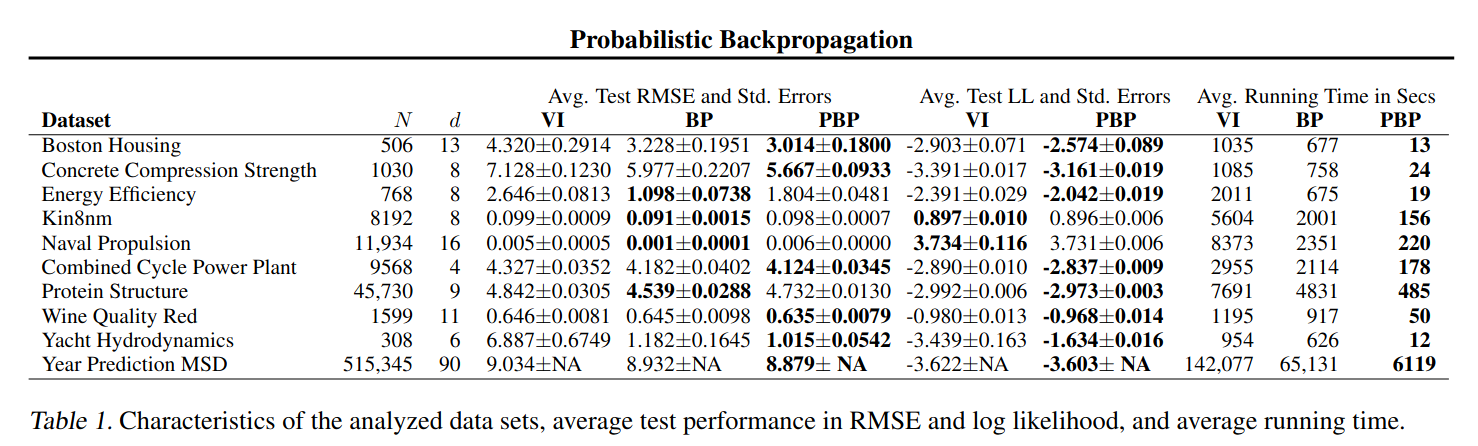
\includegraphics[width=1\textwidth, trim={0 0 0 0cm},clip]{experiments.png}
\end{figure}
\end{frame}

\begin{frame}{Literature}
\nocite{*}
\printbibliography
\end{frame}

\begin{frame}{Questions}
\textbf{1.}
Assume that the current posterior distribution for $\gamma$ is $q(\gamma) = \Gamma (\alpha^{\gamma}, \beta^{\gamma})$. After seeing new data, we update the posterior and approximate it by $q^{new}(\gamma)$. To which family of distributions does $q^{new}$ belong?

a) Gaussian

b) Gamma

c) Uniform

d) Depends on new data

\textbf{2.}
What is computed at the end of the PBP forward pass instead of the prediction error?
\end{frame}

\end{document}
